% Options for packages loaded elsewhere
\PassOptionsToPackage{unicode}{hyperref}
\PassOptionsToPackage{hyphens}{url}
%
\documentclass[
]{article}
\usepackage{amsmath,amssymb}
\usepackage{iftex}
\ifPDFTeX
  \usepackage[T1]{fontenc}
  \usepackage[utf8]{inputenc}
  \usepackage{textcomp} % provide euro and other symbols
\else % if luatex or xetex
  \usepackage{unicode-math} % this also loads fontspec
  \defaultfontfeatures{Scale=MatchLowercase}
  \defaultfontfeatures[\rmfamily]{Ligatures=TeX,Scale=1}
\fi
\usepackage{lmodern}
\ifPDFTeX\else
  % xetex/luatex font selection
\fi
% Use upquote if available, for straight quotes in verbatim environments
\IfFileExists{upquote.sty}{\usepackage{upquote}}{}
\IfFileExists{microtype.sty}{% use microtype if available
  \usepackage[]{microtype}
  \UseMicrotypeSet[protrusion]{basicmath} % disable protrusion for tt fonts
}{}
\makeatletter
\@ifundefined{KOMAClassName}{% if non-KOMA class
  \IfFileExists{parskip.sty}{%
    \usepackage{parskip}
  }{% else
    \setlength{\parindent}{0pt}
    \setlength{\parskip}{6pt plus 2pt minus 1pt}}
}{% if KOMA class
  \KOMAoptions{parskip=half}}
\makeatother
\usepackage{xcolor}
\usepackage[margin=1in]{geometry}
\usepackage{graphicx}
\makeatletter
\def\maxwidth{\ifdim\Gin@nat@width>\linewidth\linewidth\else\Gin@nat@width\fi}
\def\maxheight{\ifdim\Gin@nat@height>\textheight\textheight\else\Gin@nat@height\fi}
\makeatother
% Scale images if necessary, so that they will not overflow the page
% margins by default, and it is still possible to overwrite the defaults
% using explicit options in \includegraphics[width, height, ...]{}
\setkeys{Gin}{width=\maxwidth,height=\maxheight,keepaspectratio}
% Set default figure placement to htbp
\makeatletter
\def\fps@figure{htbp}
\makeatother
\setlength{\emergencystretch}{3em} % prevent overfull lines
\providecommand{\tightlist}{%
  \setlength{\itemsep}{0pt}\setlength{\parskip}{0pt}}
\setcounter{secnumdepth}{-\maxdimen} % remove section numbering
% definitions for citeproc citations
\NewDocumentCommand\citeproctext{}{}
\NewDocumentCommand\citeproc{mm}{%
  \begingroup\def\citeproctext{#2}\cite{#1}\endgroup}
\makeatletter
 % allow citations to break across lines
 \let\@cite@ofmt\@firstofone
 % avoid brackets around text for \cite:
 \def\@biblabel#1{}
 \def\@cite#1#2{{#1\if@tempswa , #2\fi}}
\makeatother
\newlength{\cslhangindent}
\setlength{\cslhangindent}{1.5em}
\newlength{\csllabelwidth}
\setlength{\csllabelwidth}{3em}
\newenvironment{CSLReferences}[2] % #1 hanging-indent, #2 entry-spacing
 {\begin{list}{}{%
  \setlength{\itemindent}{0pt}
  \setlength{\leftmargin}{0pt}
  \setlength{\parsep}{0pt}
  % turn on hanging indent if param 1 is 1
  \ifodd #1
   \setlength{\leftmargin}{\cslhangindent}
   \setlength{\itemindent}{-1\cslhangindent}
  \fi
  % set entry spacing
  \setlength{\itemsep}{#2\baselineskip}}}
 {\end{list}}
\usepackage{calc}
\newcommand{\CSLBlock}[1]{\hfill\break\parbox[t]{\linewidth}{\strut\ignorespaces#1\strut}}
\newcommand{\CSLLeftMargin}[1]{\parbox[t]{\csllabelwidth}{\strut#1\strut}}
\newcommand{\CSLRightInline}[1]{\parbox[t]{\linewidth - \csllabelwidth}{\strut#1\strut}}
\newcommand{\CSLIndent}[1]{\hspace{\cslhangindent}#1}
\usepackage{multirow}
\usepackage{multicol}
\usepackage{colortbl}
\usepackage{hhline}
\newlength\Oldarrayrulewidth
\newlength\Oldtabcolsep
\usepackage{longtable}
\usepackage{array}
\usepackage{hyperref}
\usepackage{float}
\usepackage{wrapfig}
\usepackage{booktabs}
\usepackage{caption}
\usepackage{anyfontsize}
\ifLuaTeX
  \usepackage{selnolig}  % disable illegal ligatures
\fi
\usepackage{bookmark}
\IfFileExists{xurl.sty}{\usepackage{xurl}}{} % add URL line breaks if available
\urlstyle{same}
\hypersetup{
  pdftitle={Estimating Missing Data's Effects on Causal Inference with Diff-in-Diff and IP-weighting},
  pdfauthor={Nathen Byford},
  hidelinks,
  pdfcreator={LaTeX via pandoc}}

\title{Estimating Missing Data's Effects on Causal Inference with
Diff-in-Diff and IP-weighting}
\author{Nathen Byford}
\date{2024-12-16}

\begin{document}
\maketitle

\section{Introduction}\label{introduction}

Missing data is a common problem among statistical analyses. Data can be
missing due to a variety of reasons, form a subject not answering a
question, to a subject leaving a study for one reason or another.
Sometimes missing data is numerous and other times a study can have no
missing data. Often times when a study has plentiful missing values
classical statistical methods using the complete cases will be biased
and something is needed to be done.

In causal inference the issue of missing data is no different, there can
be unintended bias introduced based on values that are missing. Causal
inference methods might have more or less bias introduced by missing
data due to the fact that we are trying to estimate counter factual
outcomes, outcomes that don't exist in the first place. These estimates
for the counter factual outcomes are based on the data observed in the
study and if values are missing, information about the counter factuals
is also being lost. Because of this I aim to investigate how causal
inference estimates differ when there is missing data.

\subsection{Missingness in Data}\label{missingness-in-data}

It is important to understand the different types of missing data that
can emerge in studies. Missing data can be classified into three main
types: Missing Completely at Random (MCAR), Missing at Random (MAR), and
Missing Not at Random (MNAR), each with distinct implications for
analysis Little and Rubin (2019). MCAR occurs when the missingness is
entirely unrelated to both observed and unobserved data, meaning the
data is missing purely by chance. In this case, traditional statistical
techniques like complete case analysis remain valid, as the missing data
introduces minimal bias. MAR arises when the probability of missing data
is related to observed data but not to the missing values themselves.
While this scenario introduces bias, it can often be addressed through
techniques like multiple imputation that account for the relationship
between observed variables and missingness. MNAR, on the other hand, is
the most challenging type of missing data, where the missingness is
directly related to the unobserved data. For example, patients may drop
out of a study because their condition worsens. MNAR often introduces
significant bias that cannot be addressed using standard techniques
without strong assumptions. Specialized methods, such as machine
learning-based imputation, are typically required to mitigate the impact
of MNAR data.

\section{Methods}\label{methods}

This study looks into the differences in the estimated treatment effect
for compete case analysis in MNAR data compared to the imputed data
estimated treatment effects. The following subsections go into detail
about the methods of data imputation and causal inference to estimate
the treatment effect.

\subsection{Data Imputation}\label{data-imputation}

Using Machine Learning techniques Haliduola, Bretz, and Mansmann (2022)
are able to impute MNAR data from a clinical trial for anxiety
medication. The first step of the imputation was to cluster the data by
tox response. This response curve is used to group better understand the
differences between subjects based on their initial and continued
response to the drug. Due to the time component of the data a recursive
neural network was utilized in the data imputation. In addition due to
the small sample size of some cluster over sampling was used in the
training dataset. Because of this method, the data that are MNAR can be
imputed with minimal loss of information and induced bias.

\begin{figure}
\centering
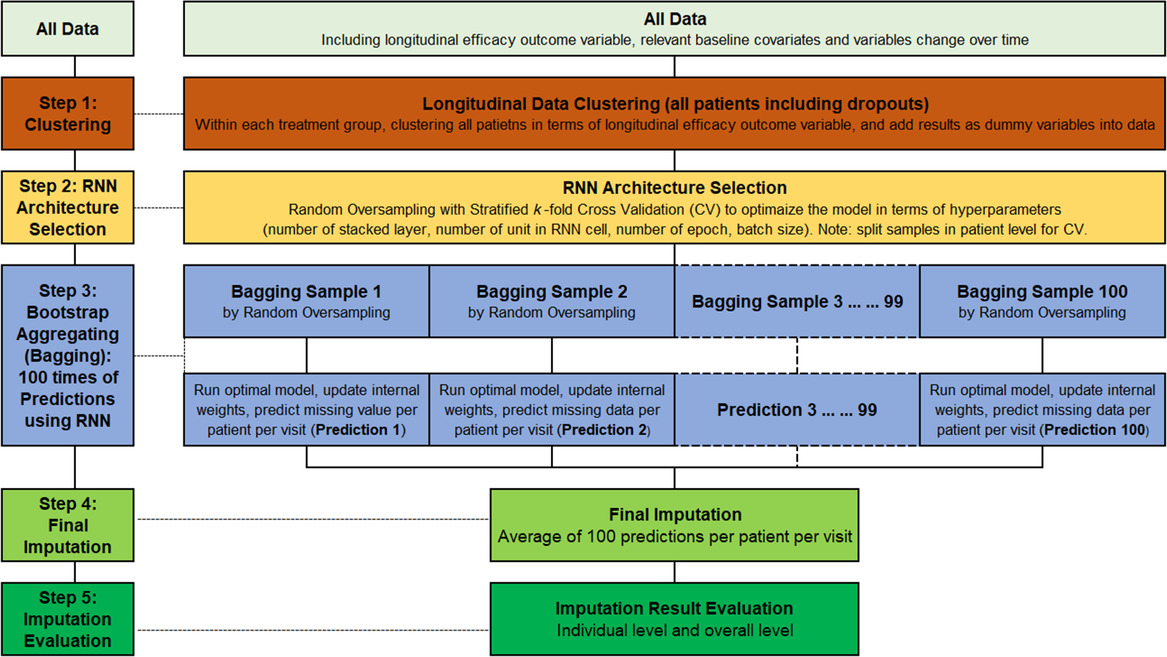
\includegraphics[width=0.6\textwidth,height=\textheight]{bimj2344-fig-0002-m.jpg}
\caption{Data Imputation Process}
\end{figure}

\subsection{Causal Inference Methods}\label{causal-inference-methods}

Two causal inference methods will be used to estimate the treatment
effect of the anxiety drug from the baseline checkup to the final
checkup. The two methods that will be tested are difference in
difference (Diff-in-Diff) and IP-weighting. Both methods estimate the
average treatment effect over time assusing that the assumptions hold.

\section{Analysis}\label{analysis}

\subsection{Exploratory Data Analysis}\label{exploratory-data-analysis}

The response variable is based on the Hamilton Anxiety Rating Scale
(HAMA), therefore a lower score represents a better response. These
scores where observed at a baseline at week 0 and then after treatment
at week 1, 2, 4, and 6. Below in figure 2 we can see the scores of each
subject at each checkup, untreated is on the left and treated subjects
are on the right. The observations shown as a red ``X'' are ones that
contain missing score values. There are 80 missing scores in the
dataset.

\begin{figure}

{\centering 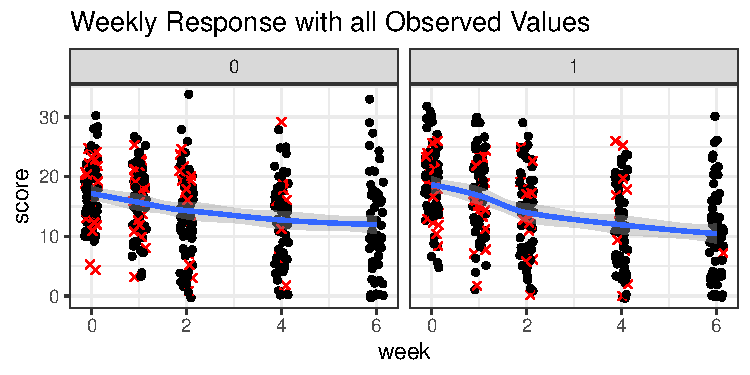
\includegraphics{missingness_in_causal_inference_files/figure-latex/unnamed-chunk-1-1} 

}

\caption{Observed responses by Week}\label{fig:unnamed-chunk-1}
\end{figure}

In the following tables we can see how these missing scores are
distributed. We can see in table 1 the split of the missing values
between treated and untreated. The split is fairly even with 38 missing
scores in the treatment group and 42 missing scores in the untreated
group. We can see that there is slightly more missing values in the
untreated group. Looking in table 2 the missing values incease as time
goes on in the study. This is possibly due to the drug potentially not
working or even the oposite. This time related missingness is a sign
that there can be a reason the data are missing and a pattern that could
be causing the missing.

\global\setlength{\Oldarrayrulewidth}{\arrayrulewidth}

\global\setlength{\Oldtabcolsep}{\tabcolsep}

\setlength{\tabcolsep}{2pt}

\renewcommand*{\arraystretch}{1.5}



\providecommand{\ascline}[3]{\noalign{\global\arrayrulewidth #1}\arrayrulecolor[HTML]{#2}\cline{#3}}

\begin{longtable}[c]{|p{0.75in}|p{0.75in}}



\ascline{1.5pt}{666666}{1-2}

\multicolumn{1}{>{\raggedleft}m{\dimexpr 0.75in+0\tabcolsep}}{\textcolor[HTML]{000000}{\fontsize{11}{11}\selectfont{Treatment}}} & \multicolumn{1}{>{\raggedleft}m{\dimexpr 0.75in+0\tabcolsep}}{\textcolor[HTML]{000000}{\fontsize{11}{11}\selectfont{NA\ count}}} \\

\ascline{1.5pt}{666666}{1-2}\endfirsthead 

\ascline{1.5pt}{666666}{1-2}

\multicolumn{1}{>{\raggedleft}m{\dimexpr 0.75in+0\tabcolsep}}{\textcolor[HTML]{000000}{\fontsize{11}{11}\selectfont{Treatment}}} & \multicolumn{1}{>{\raggedleft}m{\dimexpr 0.75in+0\tabcolsep}}{\textcolor[HTML]{000000}{\fontsize{11}{11}\selectfont{NA\ count}}} \\

\ascline{1.5pt}{666666}{1-2}\endhead



\multicolumn{1}{>{\raggedleft}m{\dimexpr 0.75in+0\tabcolsep}}{\textcolor[HTML]{000000}{\fontsize{11}{11}\selectfont{1}}} & \multicolumn{1}{>{\raggedleft}m{\dimexpr 0.75in+0\tabcolsep}}{\textcolor[HTML]{000000}{\fontsize{11}{11}\selectfont{38}}} \\





\multicolumn{1}{>{\raggedleft}m{\dimexpr 0.75in+0\tabcolsep}}{\textcolor[HTML]{000000}{\fontsize{11}{11}\selectfont{0}}} & \multicolumn{1}{>{\raggedleft}m{\dimexpr 0.75in+0\tabcolsep}}{\textcolor[HTML]{000000}{\fontsize{11}{11}\selectfont{42}}} \\

\ascline{1.5pt}{666666}{1-2}



\end{longtable}



\arrayrulecolor[HTML]{000000}

\global\setlength{\arrayrulewidth}{\Oldarrayrulewidth}

\global\setlength{\tabcolsep}{\Oldtabcolsep}

\renewcommand*{\arraystretch}{1}

\global\setlength{\Oldarrayrulewidth}{\arrayrulewidth}

\global\setlength{\Oldtabcolsep}{\tabcolsep}

\setlength{\tabcolsep}{2pt}

\renewcommand*{\arraystretch}{1.5}



\providecommand{\ascline}[3]{\noalign{\global\arrayrulewidth #1}\arrayrulecolor[HTML]{#2}\cline{#3}}

\begin{longtable}[c]{|p{0.75in}|p{0.75in}}



\ascline{1.5pt}{666666}{1-2}

\multicolumn{1}{>{\raggedleft}m{\dimexpr 0.75in+0\tabcolsep}}{\textcolor[HTML]{000000}{\fontsize{11}{11}\selectfont{Week}}} & \multicolumn{1}{>{\raggedleft}m{\dimexpr 0.75in+0\tabcolsep}}{\textcolor[HTML]{000000}{\fontsize{11}{11}\selectfont{NA\ count}}} \\

\ascline{1.5pt}{666666}{1-2}\endfirsthead 

\ascline{1.5pt}{666666}{1-2}

\multicolumn{1}{>{\raggedleft}m{\dimexpr 0.75in+0\tabcolsep}}{\textcolor[HTML]{000000}{\fontsize{11}{11}\selectfont{Week}}} & \multicolumn{1}{>{\raggedleft}m{\dimexpr 0.75in+0\tabcolsep}}{\textcolor[HTML]{000000}{\fontsize{11}{11}\selectfont{NA\ count}}} \\

\ascline{1.5pt}{666666}{1-2}\endhead



\multicolumn{1}{>{\raggedleft}m{\dimexpr 0.75in+0\tabcolsep}}{\textcolor[HTML]{000000}{\fontsize{11}{11}\selectfont{0}}} & \multicolumn{1}{>{\raggedleft}m{\dimexpr 0.75in+0\tabcolsep}}{\textcolor[HTML]{000000}{\fontsize{11}{11}\selectfont{0}}} \\





\multicolumn{1}{>{\raggedleft}m{\dimexpr 0.75in+0\tabcolsep}}{\textcolor[HTML]{000000}{\fontsize{11}{11}\selectfont{1}}} & \multicolumn{1}{>{\raggedleft}m{\dimexpr 0.75in+0\tabcolsep}}{\textcolor[HTML]{000000}{\fontsize{11}{11}\selectfont{0}}} \\





\multicolumn{1}{>{\raggedleft}m{\dimexpr 0.75in+0\tabcolsep}}{\textcolor[HTML]{000000}{\fontsize{11}{11}\selectfont{2}}} & \multicolumn{1}{>{\raggedleft}m{\dimexpr 0.75in+0\tabcolsep}}{\textcolor[HTML]{000000}{\fontsize{11}{11}\selectfont{14}}} \\





\multicolumn{1}{>{\raggedleft}m{\dimexpr 0.75in+0\tabcolsep}}{\textcolor[HTML]{000000}{\fontsize{11}{11}\selectfont{4}}} & \multicolumn{1}{>{\raggedleft}m{\dimexpr 0.75in+0\tabcolsep}}{\textcolor[HTML]{000000}{\fontsize{11}{11}\selectfont{23}}} \\





\multicolumn{1}{>{\raggedleft}m{\dimexpr 0.75in+0\tabcolsep}}{\textcolor[HTML]{000000}{\fontsize{11}{11}\selectfont{6}}} & \multicolumn{1}{>{\raggedleft}m{\dimexpr 0.75in+0\tabcolsep}}{\textcolor[HTML]{000000}{\fontsize{11}{11}\selectfont{43}}} \\

\ascline{1.5pt}{666666}{1-2}



\end{longtable}



\arrayrulecolor[HTML]{000000}

\global\setlength{\arrayrulewidth}{\Oldarrayrulewidth}

\global\setlength{\tabcolsep}{\Oldtabcolsep}

\renewcommand*{\arraystretch}{1}

\subsection{Complete Case analysis}\label{complete-case-analysis}

Using the complete cases in the dataset 80 observations are lost due to
missing response values. Using complete case analysis will most likely
result in biased estimated due to the previously mentioned MNAR nature
of the data. The goal of causal inerence is to estiamte the average
treatement effect and doing so often includes estimating counterfactual
outcomes. The estimated values of the counterfactual outcome may be
biased by the missing information in the missing data. More
sophisticated causal inference methods account for the fact that the
counterfactuals are missing themeselves and may have less bias
estimates.

The first method used is Diff-in-Diff, this method relies on the
assumptions that the treatment and control are similar with parallel
trends in the outcome. In figure 3 the trend lines for the complete case
analysis can be seen. Most importantly we can see that the trend lines
from baseline to week 1 are parallel, if there is some period before the
drug takes effect this provides evidence that the parallel trends
assumption is correct. Additionally Knowing that the data comes from a
clinical trial we can say that the the treatment and control were most
likely well randomized.

\newpage
\begin{figure}

{\centering 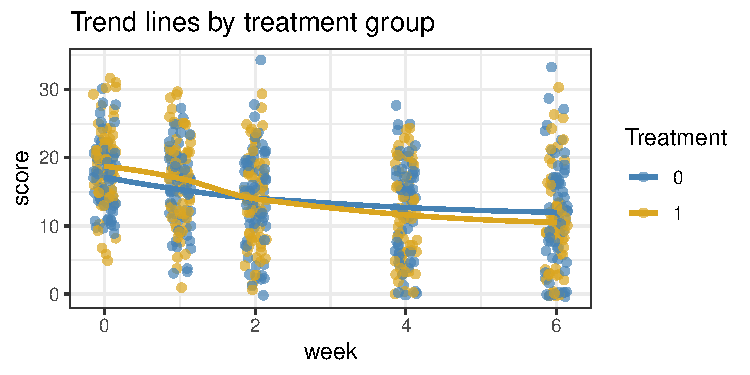
\includegraphics{missingness_in_causal_inference_files/figure-latex/unnamed-chunk-4-1} 

}

\caption{Treatment and Controll Trend Lines by Week}\label{fig:unnamed-chunk-4}
\end{figure}

Fitting the Diff-in-Diff model the results are shownin table \_\_

\begin{table}[!t]
\fontsize{12.0pt}{14.4pt}\selectfont
\begin{tabular*}{\linewidth}{@{\extracolsep{\fill}}lccc}
\toprule
\textbf{Characteristic} & \textbf{Beta} & \textbf{95\% CI}\textsuperscript{\textit{1}} & \textbf{p-value} \\ 
\midrule\addlinespace[2.5pt]
treat & 1.6 & -0.69, 3.9 & 0.2 \\ 
week & -0.86 & -1.2, -0.48 & <0.001 \\ 
DID & -0.51 & -1.1, 0.03 & 0.063 \\ 
\bottomrule
\end{tabular*}
\begin{minipage}{\linewidth}
\textsuperscript{\textit{1}}CI = Confidence Interval\\
\end{minipage}
\end{table}

\subsection{Imputed Values analysis}\label{imputed-values-analysis}

\section{Conclusion and Discussion}\label{conclusion-and-discussion}

\newpage

\section{References}\label{references}

\phantomsection\label{refs}
\begin{CSLReferences}{1}{0}
\bibitem[\citeproctext]{ref-haliduola_missing_2022}
Haliduola, Halimu N., Frank Bretz, and Ulrich Mansmann. 2022. {``Missing
Data Imputation in Clinical Trials Using Recurrent Neural Network
Facilitated by Clustering and Oversampling.''} \emph{Biometrical
Journal} 64 (5): 863--82. \url{https://doi.org/10.1002/bimj.202000393}.

\bibitem[\citeproctext]{ref-little_statistical_2019}
Little, Roderick J. A., and Donald B. Rubin. 2019. \emph{Statistical
Analysis with Missing Data}. John Wiley \& Sons.

\end{CSLReferences}

\end{document}
